\chapter{实验与评估}
\label{ch5}
之前的的章节中,我们描述了树模型鲁棒性验证框架的设计和实现过程。在本节的内容中,我们选取了一些基准的数据集在该验证框架上进行实验评估。
\section{基准数据集介绍}
我们选用了以下三个数据集评估了我们的树模型鲁棒性验证框架:
\begin{enumerate}
	\item [(1)] 波士顿房价数据集(Boston House Price Dataset)收集了在20 世纪 70 年代中期位于波士顿郊区的房屋价格的中位数,它是用于回归任务的经典数据集。该数据集有506个样本数据,每个样本数据包含了城镇人均犯罪率,高速公路便利指数,住宅的房间数等13个特征及其房屋价格的中位数。
	\item [(2)] 手写体数字识别数据集(MNIST)是用于分类任务的经典数据集,来源于美国国家标准与技术研究所。总共包含了70000个手写数字图像,每个图像的尺寸为28 x 28像素,每个像素点用灰度值表示,灰度值范围为0到255,图像分为10类别,分别代表0-9。
	\item [(3)] FASHION-MNIST 数据集包含了 70000 个不同商品的正面灰度图像,与 MNIST 数据集一样,每个图像的尺寸为28 x 28像素,灰度值范围同样为0到255。所有的图像分为10种类别,如:T恤,牛仔裤,裙子等。虽然数据集格式与 MNIST 相同,但由于图像内容的差别,使得有些模型或者算法在MNIST 和 FASHION-MNIST 的表现会有很大不同。因此对于分类任务,我们在这两个数据集上都进行了实验作为对比。
\end{enumerate}

\section{实验环境与配置}
本文中的所有的实验均在一台装有64位Ubuntu操作系统的主机上进行,所使用机器的CUP型号为Inter Core i7-5960X,主频为4.00GHz, 运行内存大小为32GB和 1T 存储硬盘大小。我们利用sklearn(scikit-learn)来训练实验中所需要的树模型:随机森林模型和GBDT 模型。sklearn 是一种开源的,基于 Python 编程语言的机器学习框架。需要注意的是,本文提出的树模型鲁棒性验证框架,同样适用于其他机器学习框架下树模型的验证(如:Silas\cite{bride2019silas},H2O,Ranger\cite{wright2015ranger} 等)。在对样本数据预处理的部分,我们使用了Pandas,Numpy 等第三方库。

\section{实验结果与分析}

\subsection{随机森林模型的鲁棒性验证与分析}

\textbf{回归模型的验证}

我们在波士顿房价数据集上展开了对随机森林回归模型的实验。在训练阶段,将数据集随机打乱,按照 4:1 的比例划分训练样本集和测试样本集。 随后利用sklearn训练出拥有不同超参数的随机森林回归模型,如:模型学习率为$\{0.1,0.2,0.3\}$,模型中树的深度为$\{5,8,10\}$,模型中树的棵树为$\{5,8,10\}$。训练出来的模型的准确率都在 $93\%$至 $98\%$之间。我们直接选取测试样本集中的样本来进行鲁棒性的验证。按照回归模型的单样本鲁棒性的定义,我们在此数据集下,对所有数据类型为数值型的特征,我们设置其对应的$\epsilon$的值为 3, $\rho$值为5代表5000美元,即在扰动房屋相关特征的情况下,模型对房屋价格的预测结果误差不能超过5000美元。

\begin{figure}[!hbt]
\centering
	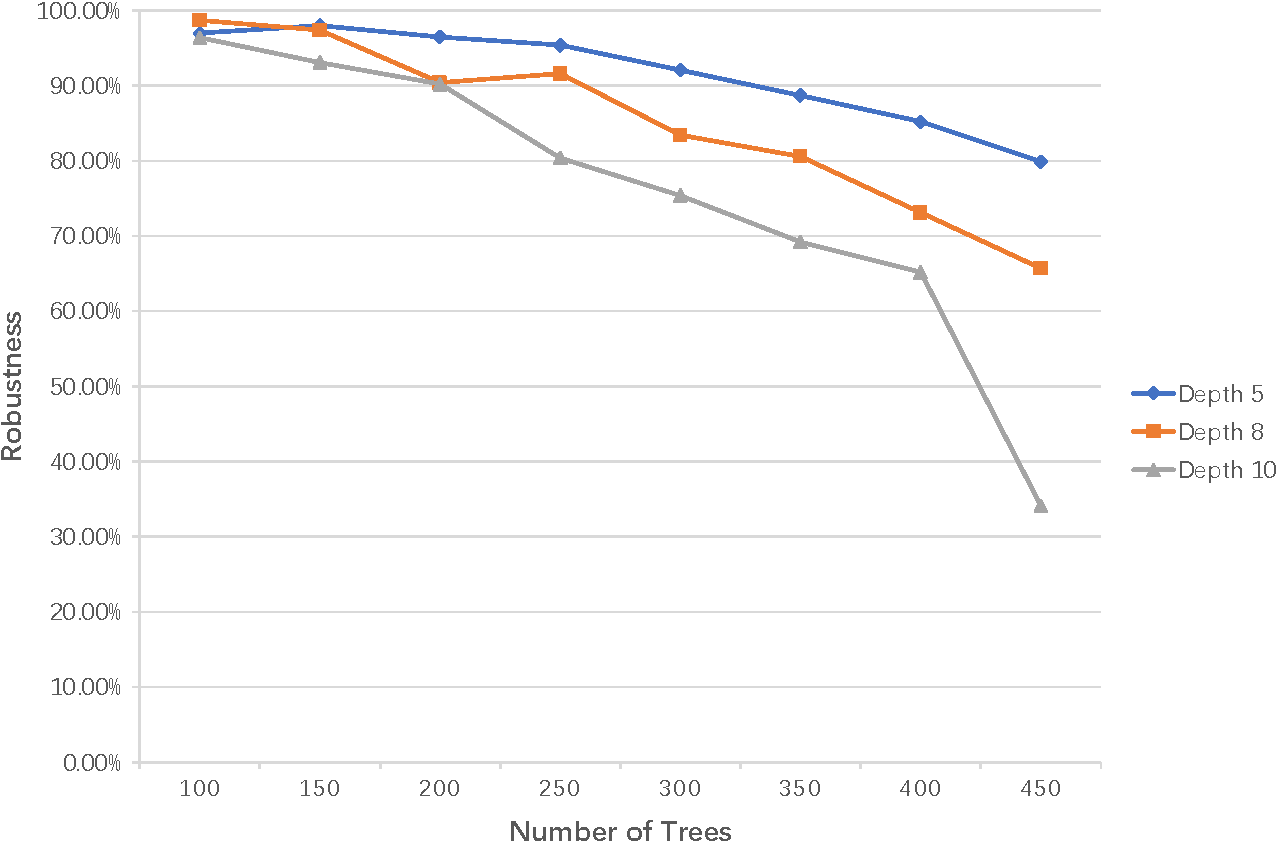
\includegraphics[scale=0.65]{fig2/C5/RF_regression_crop.pdf}
	\caption{随机森林回归模型验证结果}
	\label{fig:rf_regression}	
\end{figure}

折线图\ref{fig:rf_regression}为模型学习率为0.3下随机森林回归模型的鲁棒性验证结果。从图中我们可以看出:随着树的棵树的增加,模型的全局鲁棒性在降低而且树的深度越小,模型的鲁棒性越高。

\textbf{分类模型的验证}

对于随机森林的分类模型来说,我们分别在MNIST和FASHION-MNIST两个数据集上进行了实验验证。 对于每个数据集,首先将数据集随机打乱,将其划分为两个子集:80$\%$训练样本集和20$\%$测试样本集。 然后,我们从测试样本集中随机抽取了10个类别的各100个图像,即每个鲁棒性测试样本集的大小为1000。随后利用 sklearn训练出随机森林的分类模型,用于验证。

\begin{figure}[!hbt]
\centering
	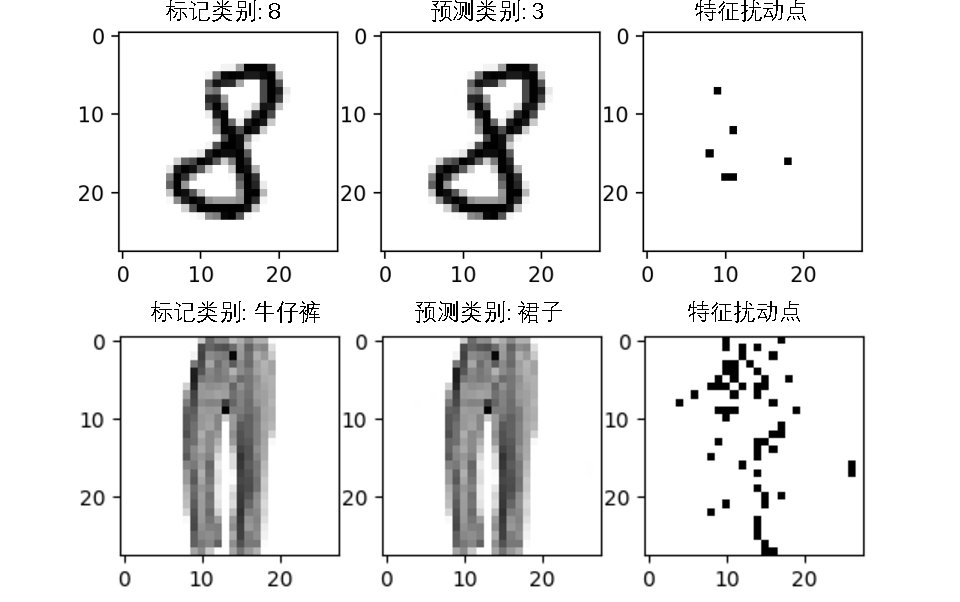
\includegraphics[scale=0.7]{fig2/C5/adversarial_example.pdf}
	\caption{对抗性样本图}
	\label{fig:adversarial_example}	
\end{figure}

图\ref{fig:adversarial_example}展示了两个数据集中不满足单样本鲁棒性的测试样本的例子。根据分类模型单样本鲁棒性的定义,我们设置特征扰动范围值$\epsilon=1$,代表了一个灰度值。图中的第一列图像为原始的样本,第二列为第一列相对应的对抗性样本图像,我们在第三列的图中标记出了受到扰动的特征点。第一个示例来源于MNIST数据集,我们可以看出在受到扰动之后,数字“ 8”被模型错误的预测为数字“3”。第二个示例来源于 FASHION-MNIST 数据集,标记类别为“牛仔裤”的商品图像被错误地分类为“裙子”。在以上示例中,如果我们直接去对比第一列的原始图像和第二列的对抗性样本图像, 凭借我们的肉眼,根本无法去找出这两个图像直接的差别(在此结果中,最多只有一个灰度值的差别)。这也反映出我们树模型鲁棒性验证框架的必要性。

\subsection{GBDT模型鲁棒性的验证与分析}
\textbf{回归模型的验证}

与随机森林的回归模型的验证实验一样,我们同样在波士顿房价数据集上进行了实验。对数据集的划分方式,训练参数的设置都与随机森林的回归模型保持一致。唯一不同的是,在 GBDT 模型中,我们需要设置损失函数,在此实验中,我们选择均方损失函数。同样,设置特征扰动范围值$\epsilon$为 3,$\rho$值为5,代表5000美元,即在房屋特征扰动的情况下,此模型对房屋价格的预测结果误差不能超过5000美元。

\begin{figure}[!hbt]
\centering
	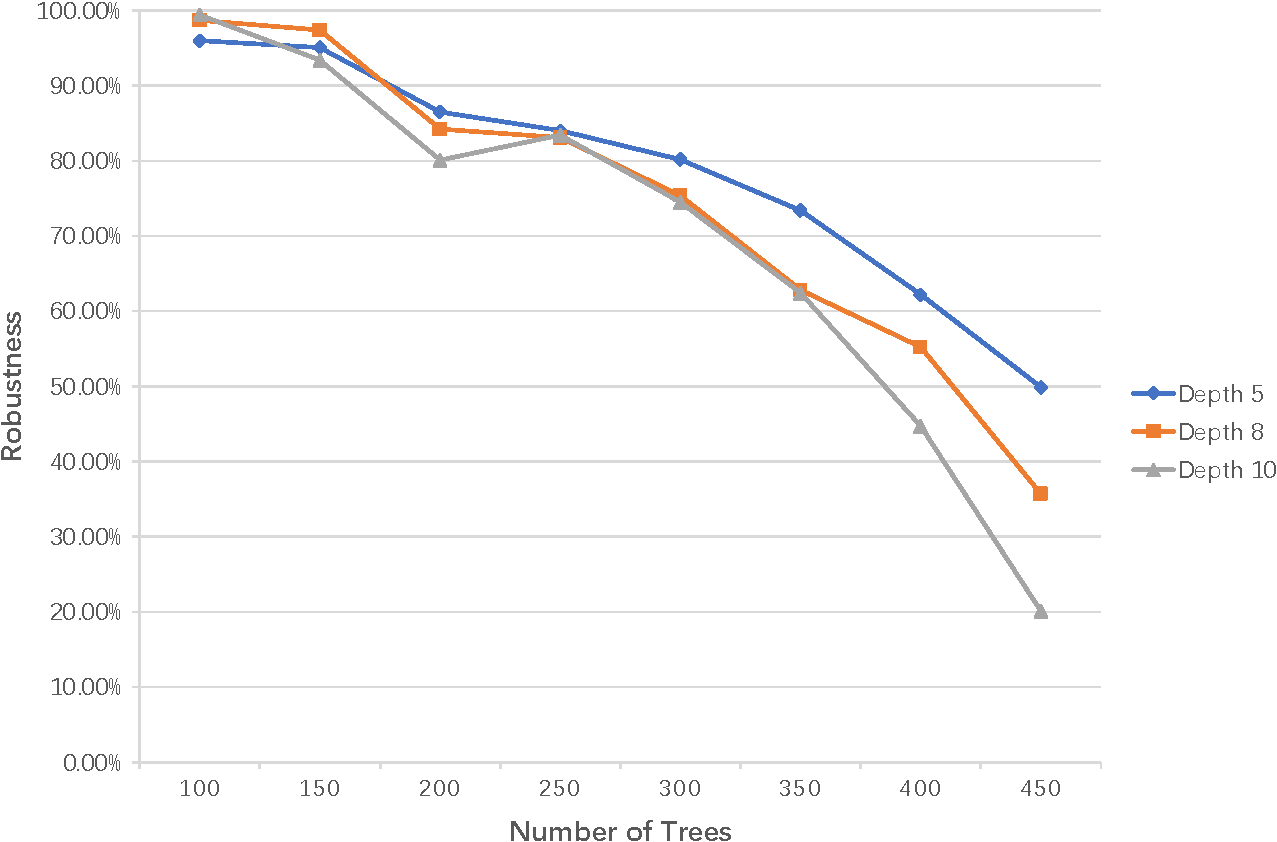
\includegraphics[scale=0.65]{fig2/C5/gb/gb_regression.pdf}
	\caption{GBDT回归模型验证结果}
	\label{fig:GBDT回归验证}	
\end{figure}

图\ref{fig:GBDT回归验证}为模型学习率为0.3下GBDT回归模型的鲁棒性验证结果。从图中我们可以看出,与随机森林回归模型一致,随着树的深度和树的棵树的增加,模型的全局鲁棒性在降低。但在增加同样棵树的决策树情况下,GBDT 的回归模型的鲁棒性要比随机森林模型下降的更快。换句话说,随机森林模型鲁棒性的下降趋势较为“平缓”,而GBDT 模型鲁棒性的下降趋势则比较“陡峭”。

\textbf{分类模型的验证}

在 GBDT 分类模型的鲁棒性验证实验中,我们同样基于MNIST和FASHION-MNIST两个数据集上进行了实验验证。数据集的划分方式为:80$\%$训练样本集和20$\%$测试样本集。之后,从测试样本集中随机抽取了10个类别的各100个图像,总的鲁棒性测试样本集的大小为1000。

\begin{figure}[!hbt]
\centering
	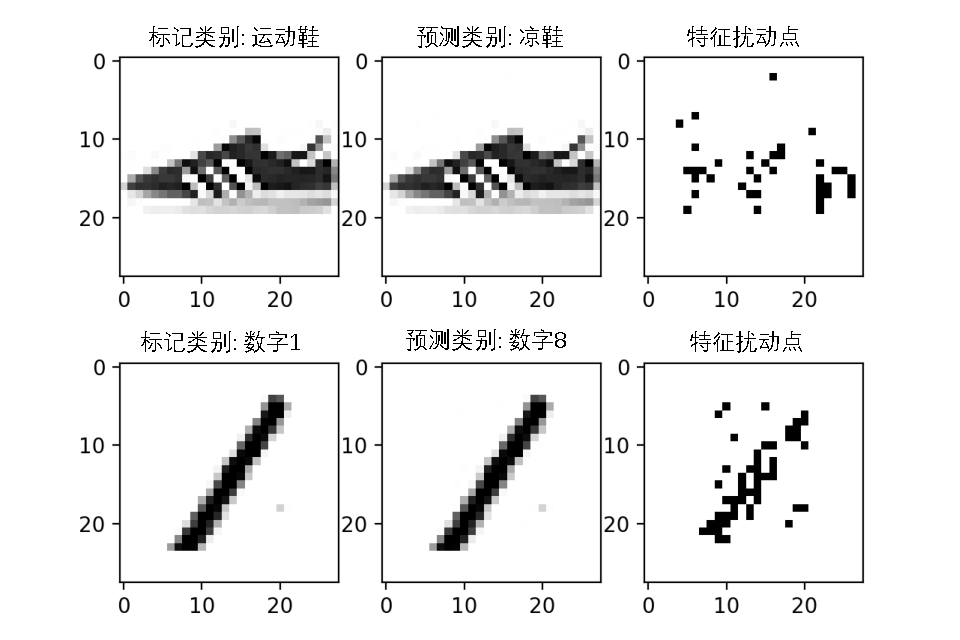
\includegraphics[scale=0.7]{fig2/C5/gb/gb_ad.pdf}
	\caption{GBDT验证反例}
	\label{fig:GBDT验证反例}	
\end{figure}

图\ref{fig:GBDT验证反例}显示了 GBDT 分类模型下不满足单样本鲁棒性的测试样本。其特征扰动范围值$\epsilon=3$,即最多扰动3个灰度值。图中的第一列图像为原始的样本,第二列为第一列相对应的对抗性样本图像,第三列的图像标记出了受到扰动的特征点。我们可以看出在图像受到扰动之后,在第一个示例中标记为类别“运动鞋”的商品图像被错误地预测为“凉鞋”。第二个示例中数字“1”被模型错误的预测为数字“8”。在扰动范围设置为 3 个灰度值的情况下,我们依然无法通过肉眼看出原始图像和对抗性样本图像之间的区别。

\subsection{树模型鲁棒性可解释性的实验与分析}
\textbf{鲁棒特征集合}

根据我们给出的鲁棒特征集合定义,我们在随机森林分类模型和 GBDT 分类模型中,进行了相关的实验与分析。根据定义可知,在测试样本满足单样本鲁棒性的情况下,我们可以获取其鲁棒特征集合。因此,我们可以直接在之前分类模型的实验中,获取满足鲁棒性的样本的鲁棒特征集合。

\begin{figure}[!hbt]
\centering
	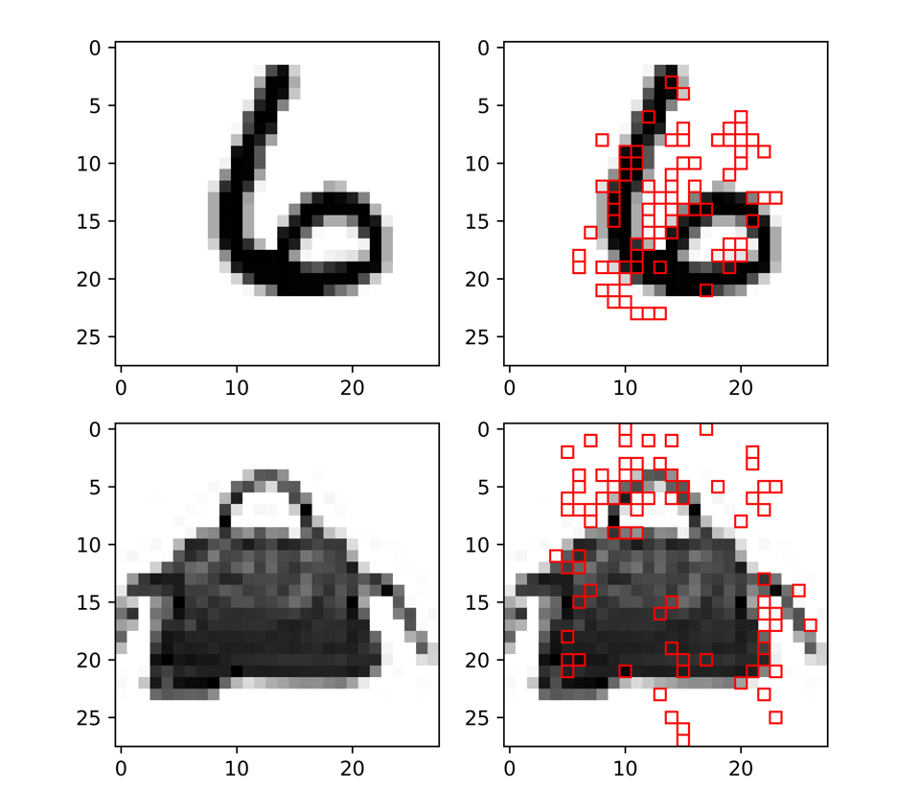
\includegraphics[scale=0.5]{fig2/C5/robust_feature_set.png}
	\caption{随机森林分类模型鲁棒特征集合}
	\label{fig:robust_feature_set}	
\end{figure}

图\ref{fig:robust_feature_set}显示了在随机森林分类模型下的两个数据集中满足单样本鲁棒性的测试样本的示例。特征扰动范围$\epsilon$设置为3,代表了 3 个灰度值。在受到扰动的情况下,这些样本仍然被模型正确识别。图中的第一列显示了原始的样本,第二列为对应图像的鲁棒特征集合图。我们用红色矩形标记处了存在于该样本鲁棒特征集合中的特征点。根据鲁棒特征集合的性质,我们知道保持红色矩形标记的特征点的像素灰度值不变,在特征扰动距离最大为3个灰度值的情况下任意改变其他特征点的像素灰度值都不能改变模型对该样本的识别结果。为了验证此结论,我们随机的改变不包含于鲁棒特征集合中的特征点的像素灰度值,而保持红色标记点像素灰度值不变,然后让模型去识别将改变后的测试样本之后,去检查预测结果是否发生变化。经过大量的随机测试,以上结论正确。

\begin{figure}[!hbt]
\centering
	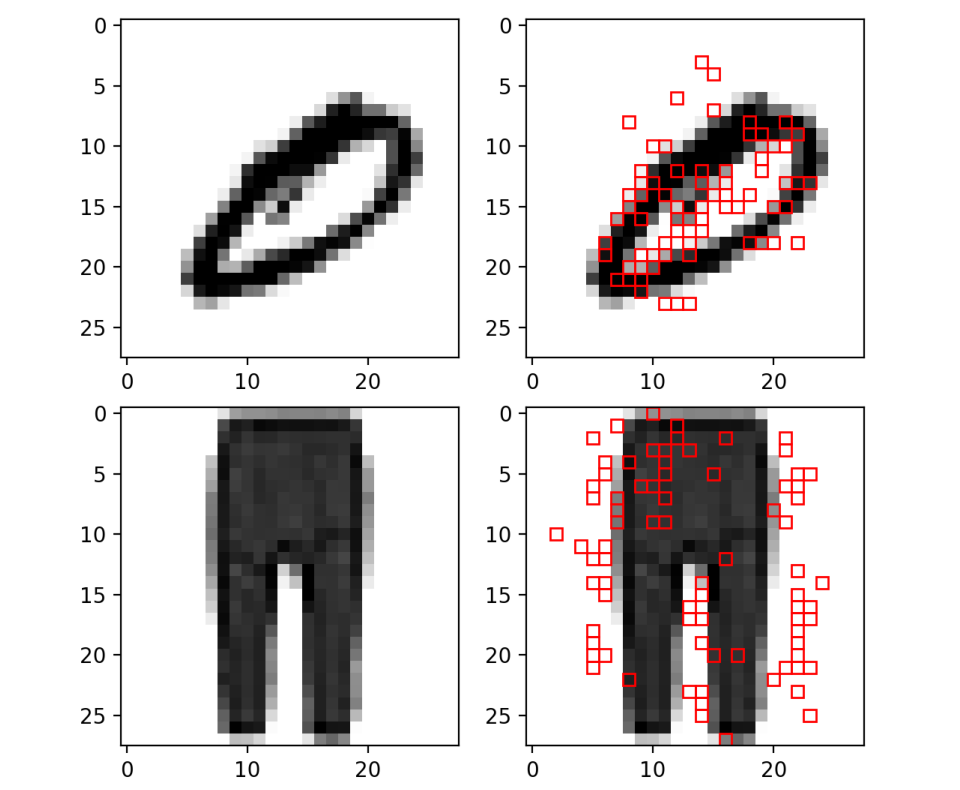
\includegraphics[scale=0.5]{fig2/C5/gb/gb_RFS.pdf}
	\caption{GBDT分类模型鲁棒特征集合}
	\label{fig:gb_robust_feature_set}	
\end{figure}

图\ref{fig:gb_robust_feature_set}显示了在GBDT分类模型下的两个数据集中满足单样本鲁棒性的测试样本的示例。特征扰动范围$\epsilon$设置为1。实验过程与随机森林实验保持一致。第一行显示的为数字“0”样本的鲁棒特征集合,第二行显示的为商品“裤子”样本的结果。

\textbf{局部鲁棒特征重要度}

根据我们对局部鲁棒特征重要度的定义,我们首先收集了的在随机森林分类模型测试样本集中所有满足单样本鲁棒性的测试样本,根据算法\ref{LRFI algorithm},我们们可以求得模型不同类别的鲁棒特征重要度。

\begin{figure}[!hbt]
\centering
	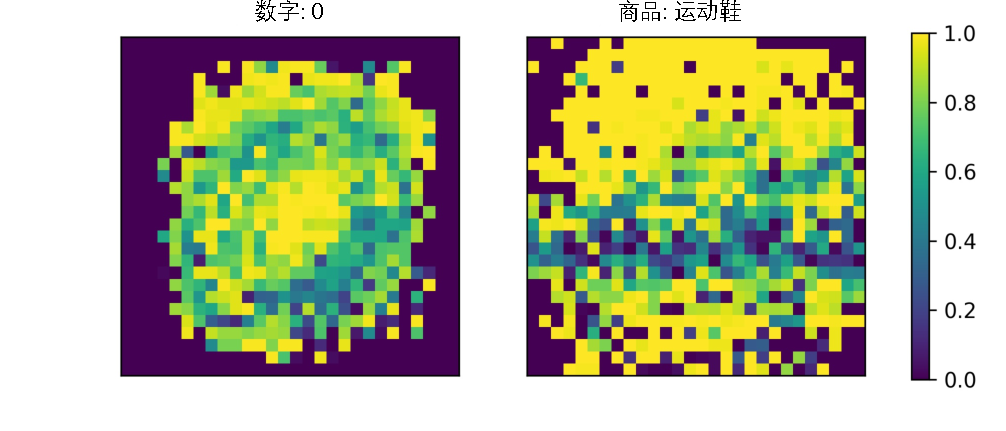
\includegraphics[scale=0.7]{fig2/C5/LBTZ.pdf}
	\caption{随机森林分类的局部鲁棒性特征重要度}
	\label{fig:LRFI}	
\end{figure}

我们在分别在 MNIST 和 FAHSION-MNIST 数据集中,各自选择了一个类别来计算局部鲁棒特征重要度。图\ref{fig:LRFI}展示了基于随机森林分类模型的实验结果。左侧的图片为MNIST中数字“ 0”的结果,右侧显示了FASHION-MNIST中的商品“ 运动鞋”的结果。特征点的鲁棒重要度的值越大,则颜色越黄。如果其鲁棒重要度的值为0,则颜色为紫色。我们可以观察到由于特征点的重要度值的不同,显示出了该类别的基本形状。重要度大的值基本分布在该类别的基本形状周围,而分布在该类别的基本形状之上的特征点的鲁棒重要度值都比较低。这为对抗性样本的攻击提供了新的思路:在进行对抗性样本攻击的时候,应该优先选择这些鲁棒重要度值比较高的点,去产生对抗性样本,这样可以提高攻击的成功率与效率。如果从我们实验得出的特征重要度分布的规律来看,应该优先选择分布在该类别基本形状周围的特征点去进行攻击。需要注意的是,除了我们给出的以上两个类别的结果之外,其他类别的鲁棒特征重要度也有类似的分布规律。

\subsection{不同类别鲁棒性的验证与分析}

在其他关于树模型的鲁棒性的验证研究中,对于分类模型的鲁棒性验证都是针对于该模型的整体而言的。但是同一模型的不同的类别的鲁棒性可能会不同。在此种情况下,整体的模型鲁棒性的验证结果,并不能提供具体类别的鲁棒性信息。所以我们设计了实验去研究同一模型下不同类别的鲁棒性的是否会出现差异的问题。与之前的实验设置保持一致,数据集的划分方式为:80$\%$训练样本集和20$\%$测试样本集,从测试样本集中随机抽取了10个类别的各100个图像。训练出的树模型的识别率都在 95$\%$ 至 98$\%$之间,并且各个类别的识别率也基本相同。之后我们分别对不同类别的 100 个样本进行鲁棒性验证。

\begin{figure}[!hbt]
\centering
        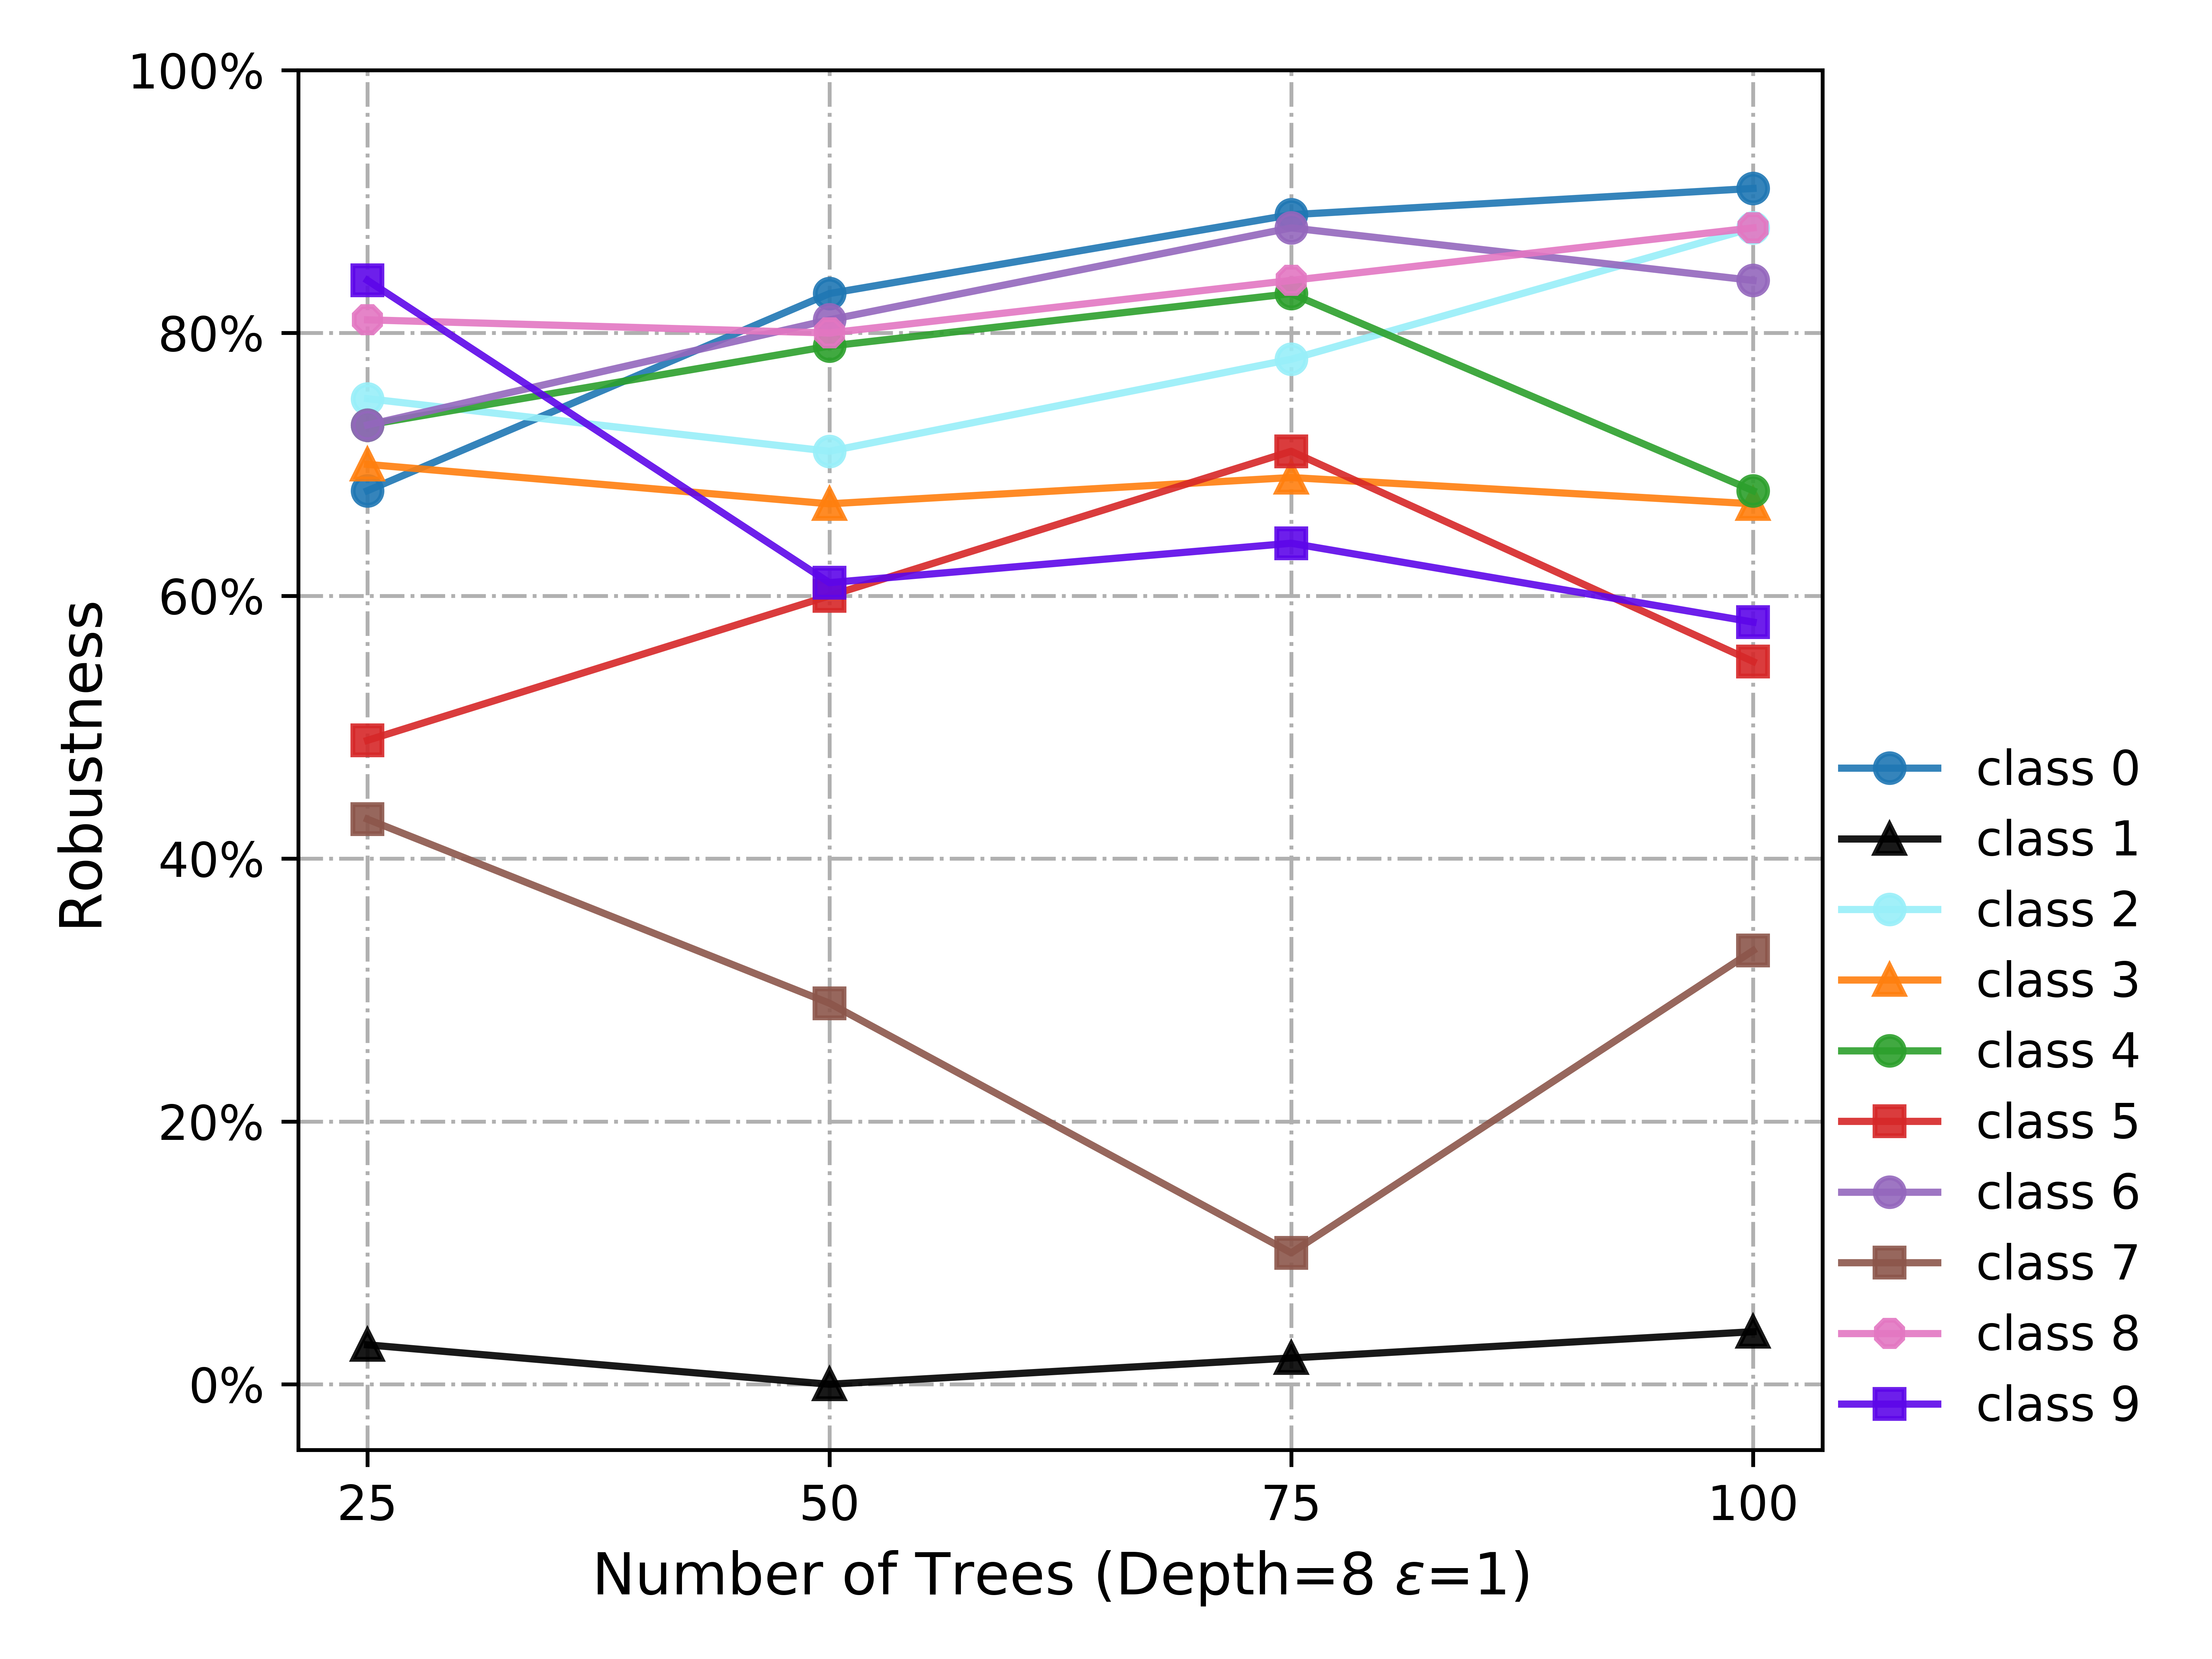
\includegraphics[scale=0.65]{fig2/C5/mnist_com.png}
	\caption{MNIST 中不同类别鲁棒性的验证结果}
	\label{fig:MNIST不同}	
\end{figure}

\begin{figure}[!hbt]
\centering
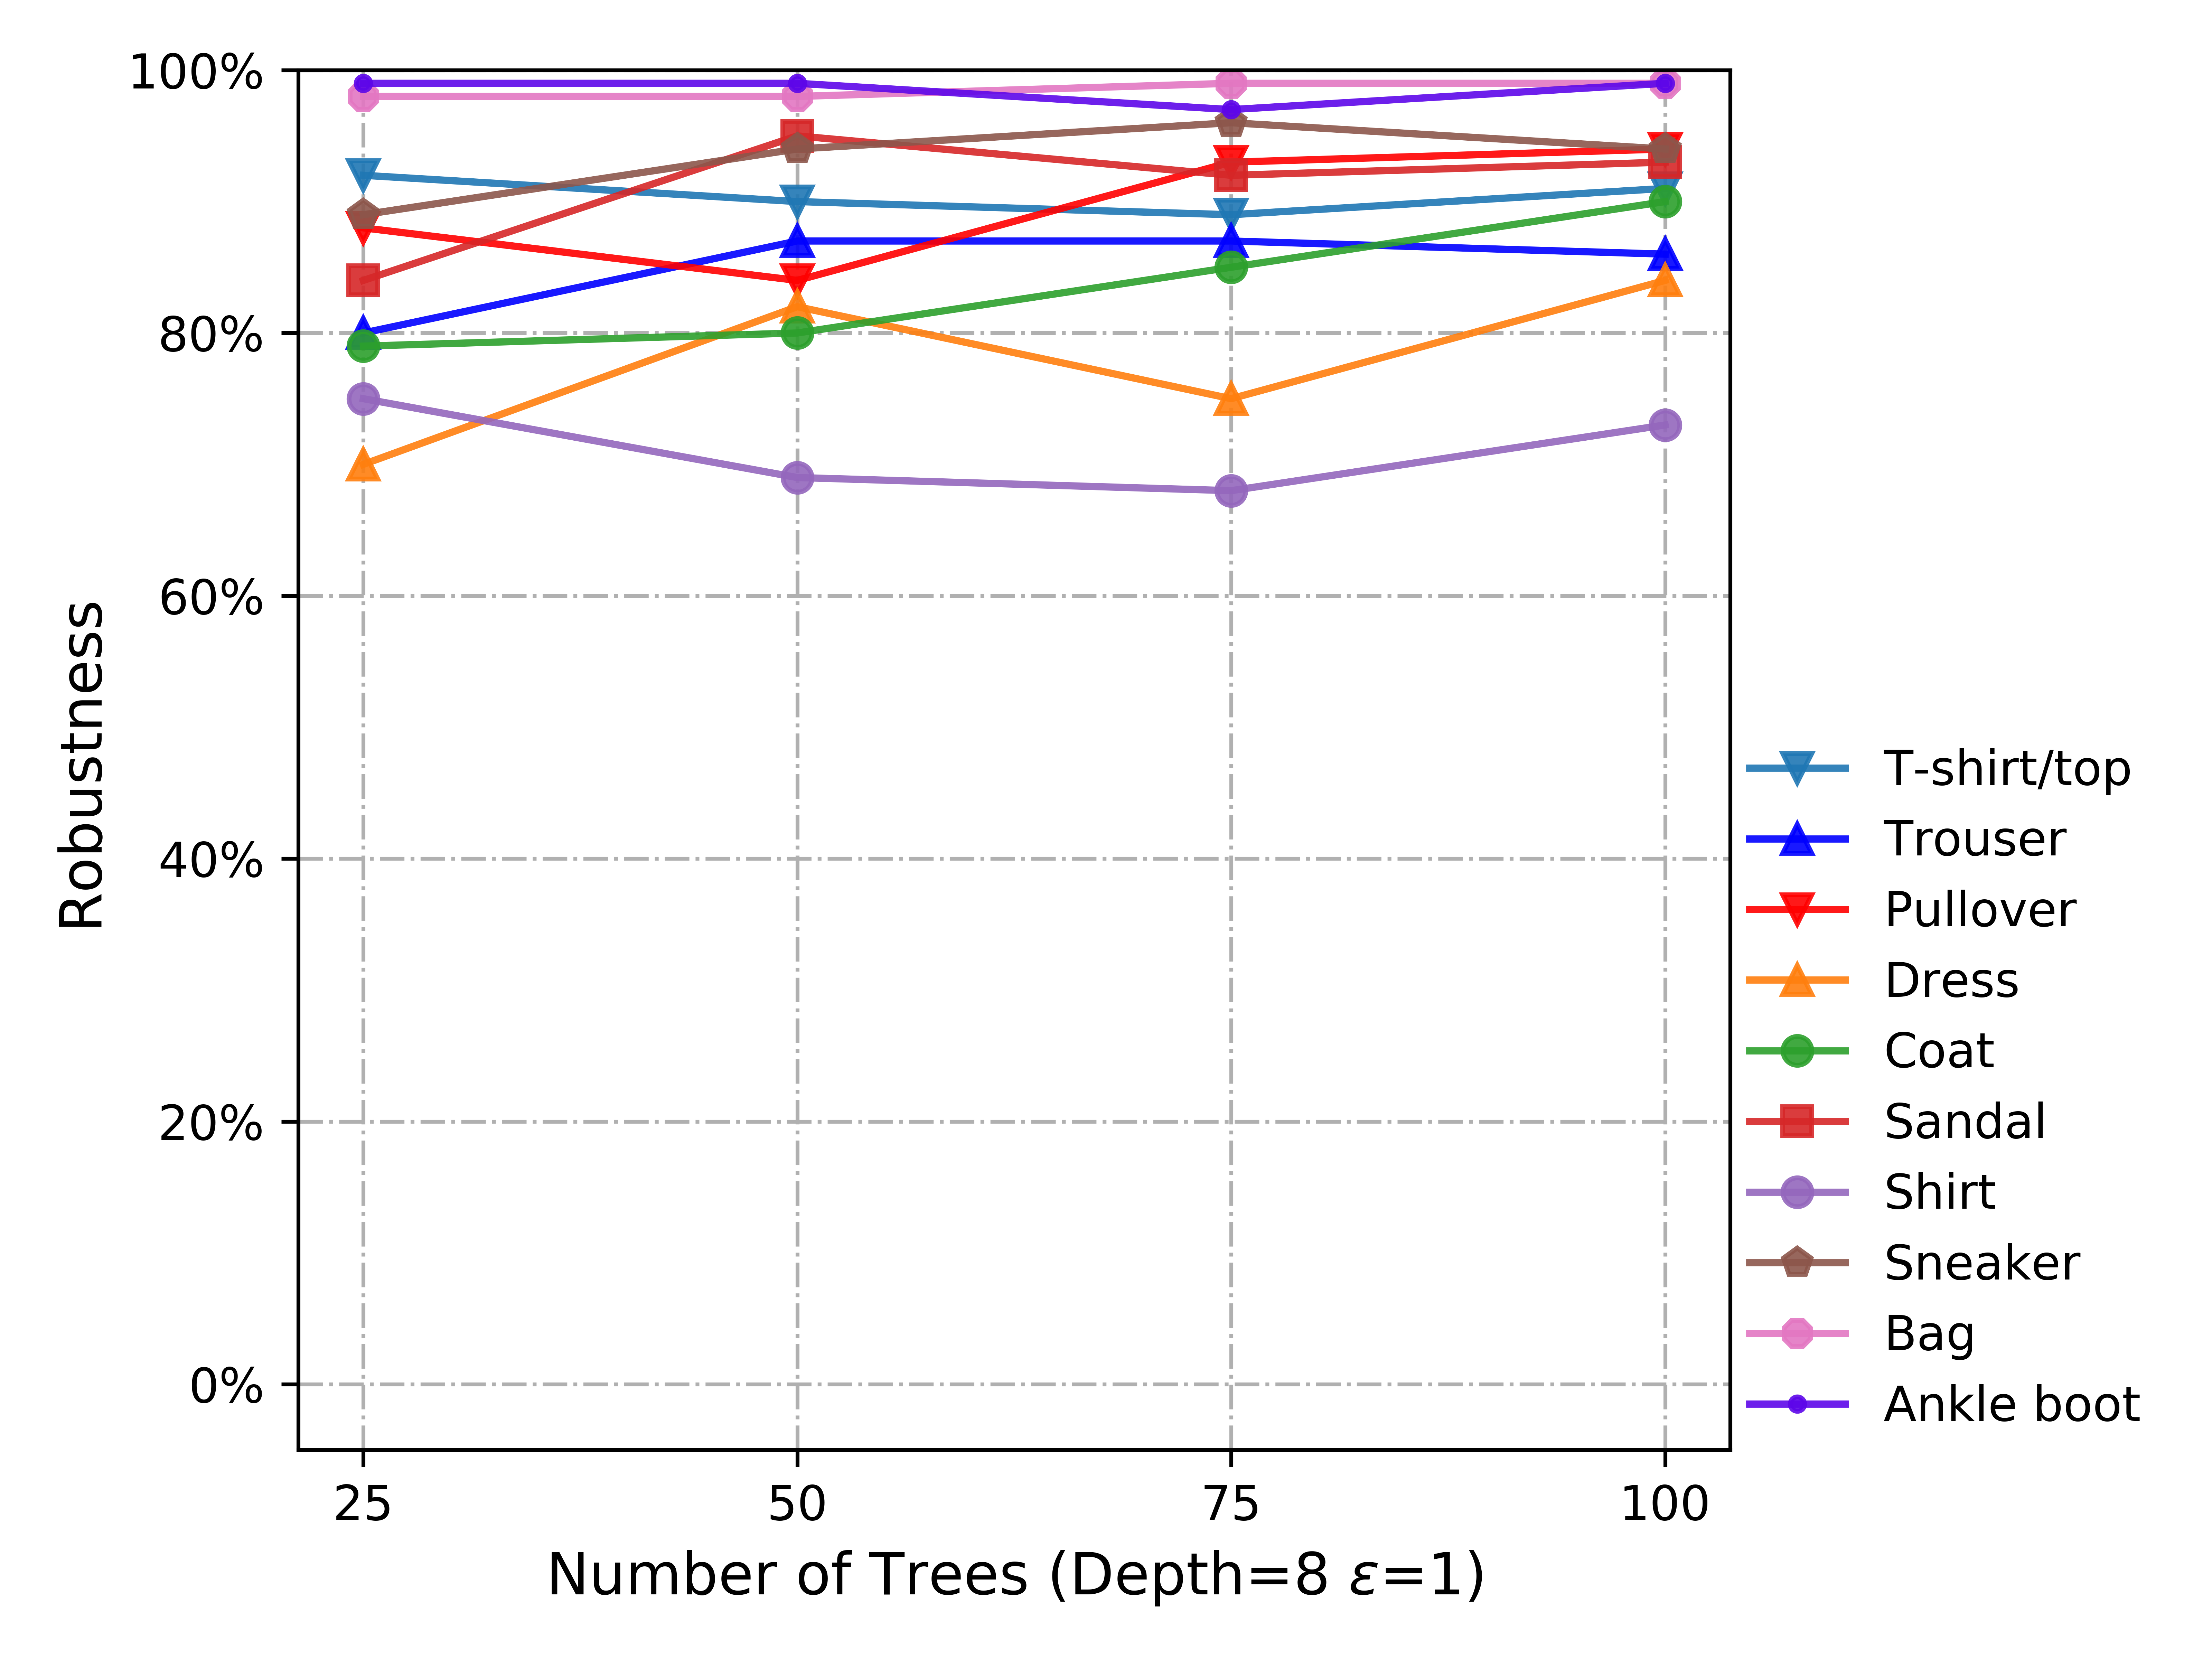
\includegraphics[scale=0.7]{fig2/C5/fashion_com.png}
	\caption{FASHION-MNIST 中不同类别鲁棒性的验证结果}
	\label{fig:Fashion不同}	
\end{figure}



折线图\ref{fig:MNIST不同}和\ref{fig:Fashion不同}展示了两个数据集中的不同类别的鲁棒性验证结果。图\ref{fig:MNIST不同}显示了MNIST数据集的结果。我们可以观察到,存在几个类别(例如,数字“ 0”,数字“ 2”,数字“ 6”,数字“ 8”)的鲁棒性随着树的棵树的增加而略有提高。而数字“ 4”,数字“ 5”,数字“ 7”,数字“ 9”类中的鲁棒性值有很明显的波动。除此以外,数字“ 1”的鲁棒性始终保持在非常低的值。 尽管模型对数字“1”的识别率与其他数字的识别率基本一样,但它们的鲁棒性值却存在着显着差异,差值大约在40$\%$至80$\%$之间。相比之下,FASHION-MNIST(图\ref{fig:Fashion不同})中各个类别的鲁棒性总体上保持稳定,并没有随着树的棵树的增加而出现明显的波动。但是,商品类别为“衬衫”的鲁棒性值相比于其他类别要低一些。在该数据集中,没有类似于数字“1”这种的鲁棒性非常低的类别去影响该模型的总体的鲁棒性值。根据此次的实验结果,我们可知在验证树模型鲁棒性的时候,将注意力集中在整个模型的鲁棒性上是不准确的,对于不同的数据集来说,模型对于不同类别样本的鲁棒性的表现可能会有很大的差别。这给了我们的一个启示,在验证在验证分类模型鲁棒性的时候,验证结果应该细化到不同的类别。这些信息对于模型的使用者来说是非常有用的,可以让他们更加详细的了解到该模型的优缺点,从而增加了模型的可信度。

\subsection{树鲁棒性超参数与鲁棒性关系的验证与分析}

在本文提出的鲁棒性验证框架下,我们进一步研究了树模型中两个重要的训练超参数:树的棵树和树的深度与树模型鲁棒性的关系。我们基于 MNIST 数据集去进行这部分的实验。通过在不同深度,不同树的棵树参数下去训练模型,通过对比其鲁棒性结果来进行研究和分析。
\begin{table*}
\caption{基于MNIST 数据集模型在不同超参数下的鲁棒性验证结果.}
\begin{center}
\begin{tabular}{|c|c|c|c|c|c|c|c|c|c|c|}
\hline 
\multirow{2}{*}{Trees} & \multirow{2}{*}{Depth} & \multirow{2}{*}{Accuracy} & \multicolumn{3}{c|}{$\epsilon=1$} &  \multicolumn{3}{c|}{$\epsilon=3$} \\ \cline{4-9}
& & & Verified($\rho$) & Timeout & Failed & Verified($\rho$) & Timeout & Failed \\
\hline
25 & 5& 84$\%$&45.71$\%$ &0$\%$ &54.29$\%$& 9.64$\%$& 0.12$\%$& 90.24$\%$ \\
\hline
50& 5& 85$\%$&54.68$\%$ &0$\%$ &45.32$\%$ & 13.58$\%$&2.69$\%$ & 83.72$\%$ \\
\hline
75& 5& 86$\%$& 48.77$\%$&5.61$\%$ &45.61$\%$ &9.24$\%$ & 13.68$\%$&77.08$\%$  \\
\hline
100&5 & 86$\%$& 54.07$\%$& 14.53$\%$& 31.40$\%$&13.02$\%$ &21.74$\%$ &65.23$\%$  \\
\hline
25& 8& 91$\%$& 61.47$\%$& 0$\%$& 38.53$\%$&9.88$\%$ &0.11$\%$ &90.01$\%$  \\
\hline
50& 8& 93$\%$& 61.02$\%$&0$\%$ &38.98$\%$ &14.36$\%$ &3.02$\%$ &82.61$\%$  \\
\hline
75& 8& 92$\%$& 63.63$\%$&5.32$\%$ &31.05$\%$ &12.81$\%$ &17.05$\%$ &70.14$\%$  \\
\hline
100& 8& 93$\%$& 63.48$\%$&15.04$\%$ &21.48$\%$ & 16.86$\%$&24.81$\%$ &58.32$\%$  \\
\hline
25&10 & 93$\%$& 64.34$\%$& 0$\%$& 35.66$\%$& 14.18$\%$& 0$\%$&85.82$\%$  \\
\hline
50& 10& 95$\%$& 63.21$\%$&0$\%$ & 36.79$\%$&17.34$\%$ &0.53$\%$ &82.14$\%$  \\
\hline
75& 10& 94$\%$& 75.32$\%$&5.32$\%$ & 19.36$\%$& 13.83$\%$& 4.57$\%$&81.60$\%$  \\
\hline
100& 10& 95$\%$& 66.84$\%$& 8.74$\%$& 24.42$\%$&15.16$\%$ &14.21$\%$ &70.63$\%$  \\
\hline
\end{tabular}
\label{tab1}
\end{center}
\end{table*}

表\ref{tab1}为随机森林分类模型在不同训练参数下的鲁棒性结果,其中 Trees 和 Depth 分别表示模型中树的棵树和树的深度,Acrruracy 表示的是模型的识别率,Verified($\rho$)表示模型的全局鲁棒性,Timeout 表示验证超时,Failed 表示验证失败即不满足单样本鲁棒性所占的百分比。我们可以观察到,在特征扰动值为$\epsilon=1$的情况下,保持相同树的深度,树的棵树并不会对其鲁棒性造成很大的影响,但在之前的对回归模型的实验中,在保持树的深度相同的情况下,树的棵树的增加,会导致其模型鲁棒性的降低。
此外,在保持树的棵树相同的情况下,增加树的深度参数的值,会使模型的鲁棒性少量的增加。与之相反的是,对于其回归模型来说,树的深度的增加,会导致其模型鲁棒性的降低。根据我们的实验结果,在保证模型准别率的情况下,模型的开发人员可以通过调整训练参数来增加其模型的鲁棒性。与$\epsilon=1$时做对比,$\epsilon=3$的情况下,该模型的鲁棒性有了明显的降低,这是显而易见的,因为在特征扰动范围为 3 个灰度值的情况下,会产生更多的对抗性样本使得原始样本的鲁棒性不满足。

还有一点值得我们注意,随着树的棵树和树的深度的值的增加,验证超时的比例也在增加,这揭露了我们验证框架的不足。因为从本质上来说,验证框架的验证能力一定程度取决于 Z3 求解器的求解能力,当树模型规模变大的时候,我们编码形成的 SMT 公式数目也是剧增的,这就导致状态爆炸的问题,从而使得求解器无法求解,导致验证超时,无法确定该样本的鲁棒性是否满足。

\subsection{验证时间的结果与分析}
框架的验证时间同样也是我们需要关注的部分,我们需要保证在一定时间内返回正确的验证结果。于是,我们基于 MNIST 数据集,通过验证不同规模大小的树模型来统计该框架的验证时间。
\begin{figure}[!hbt]
\centering
	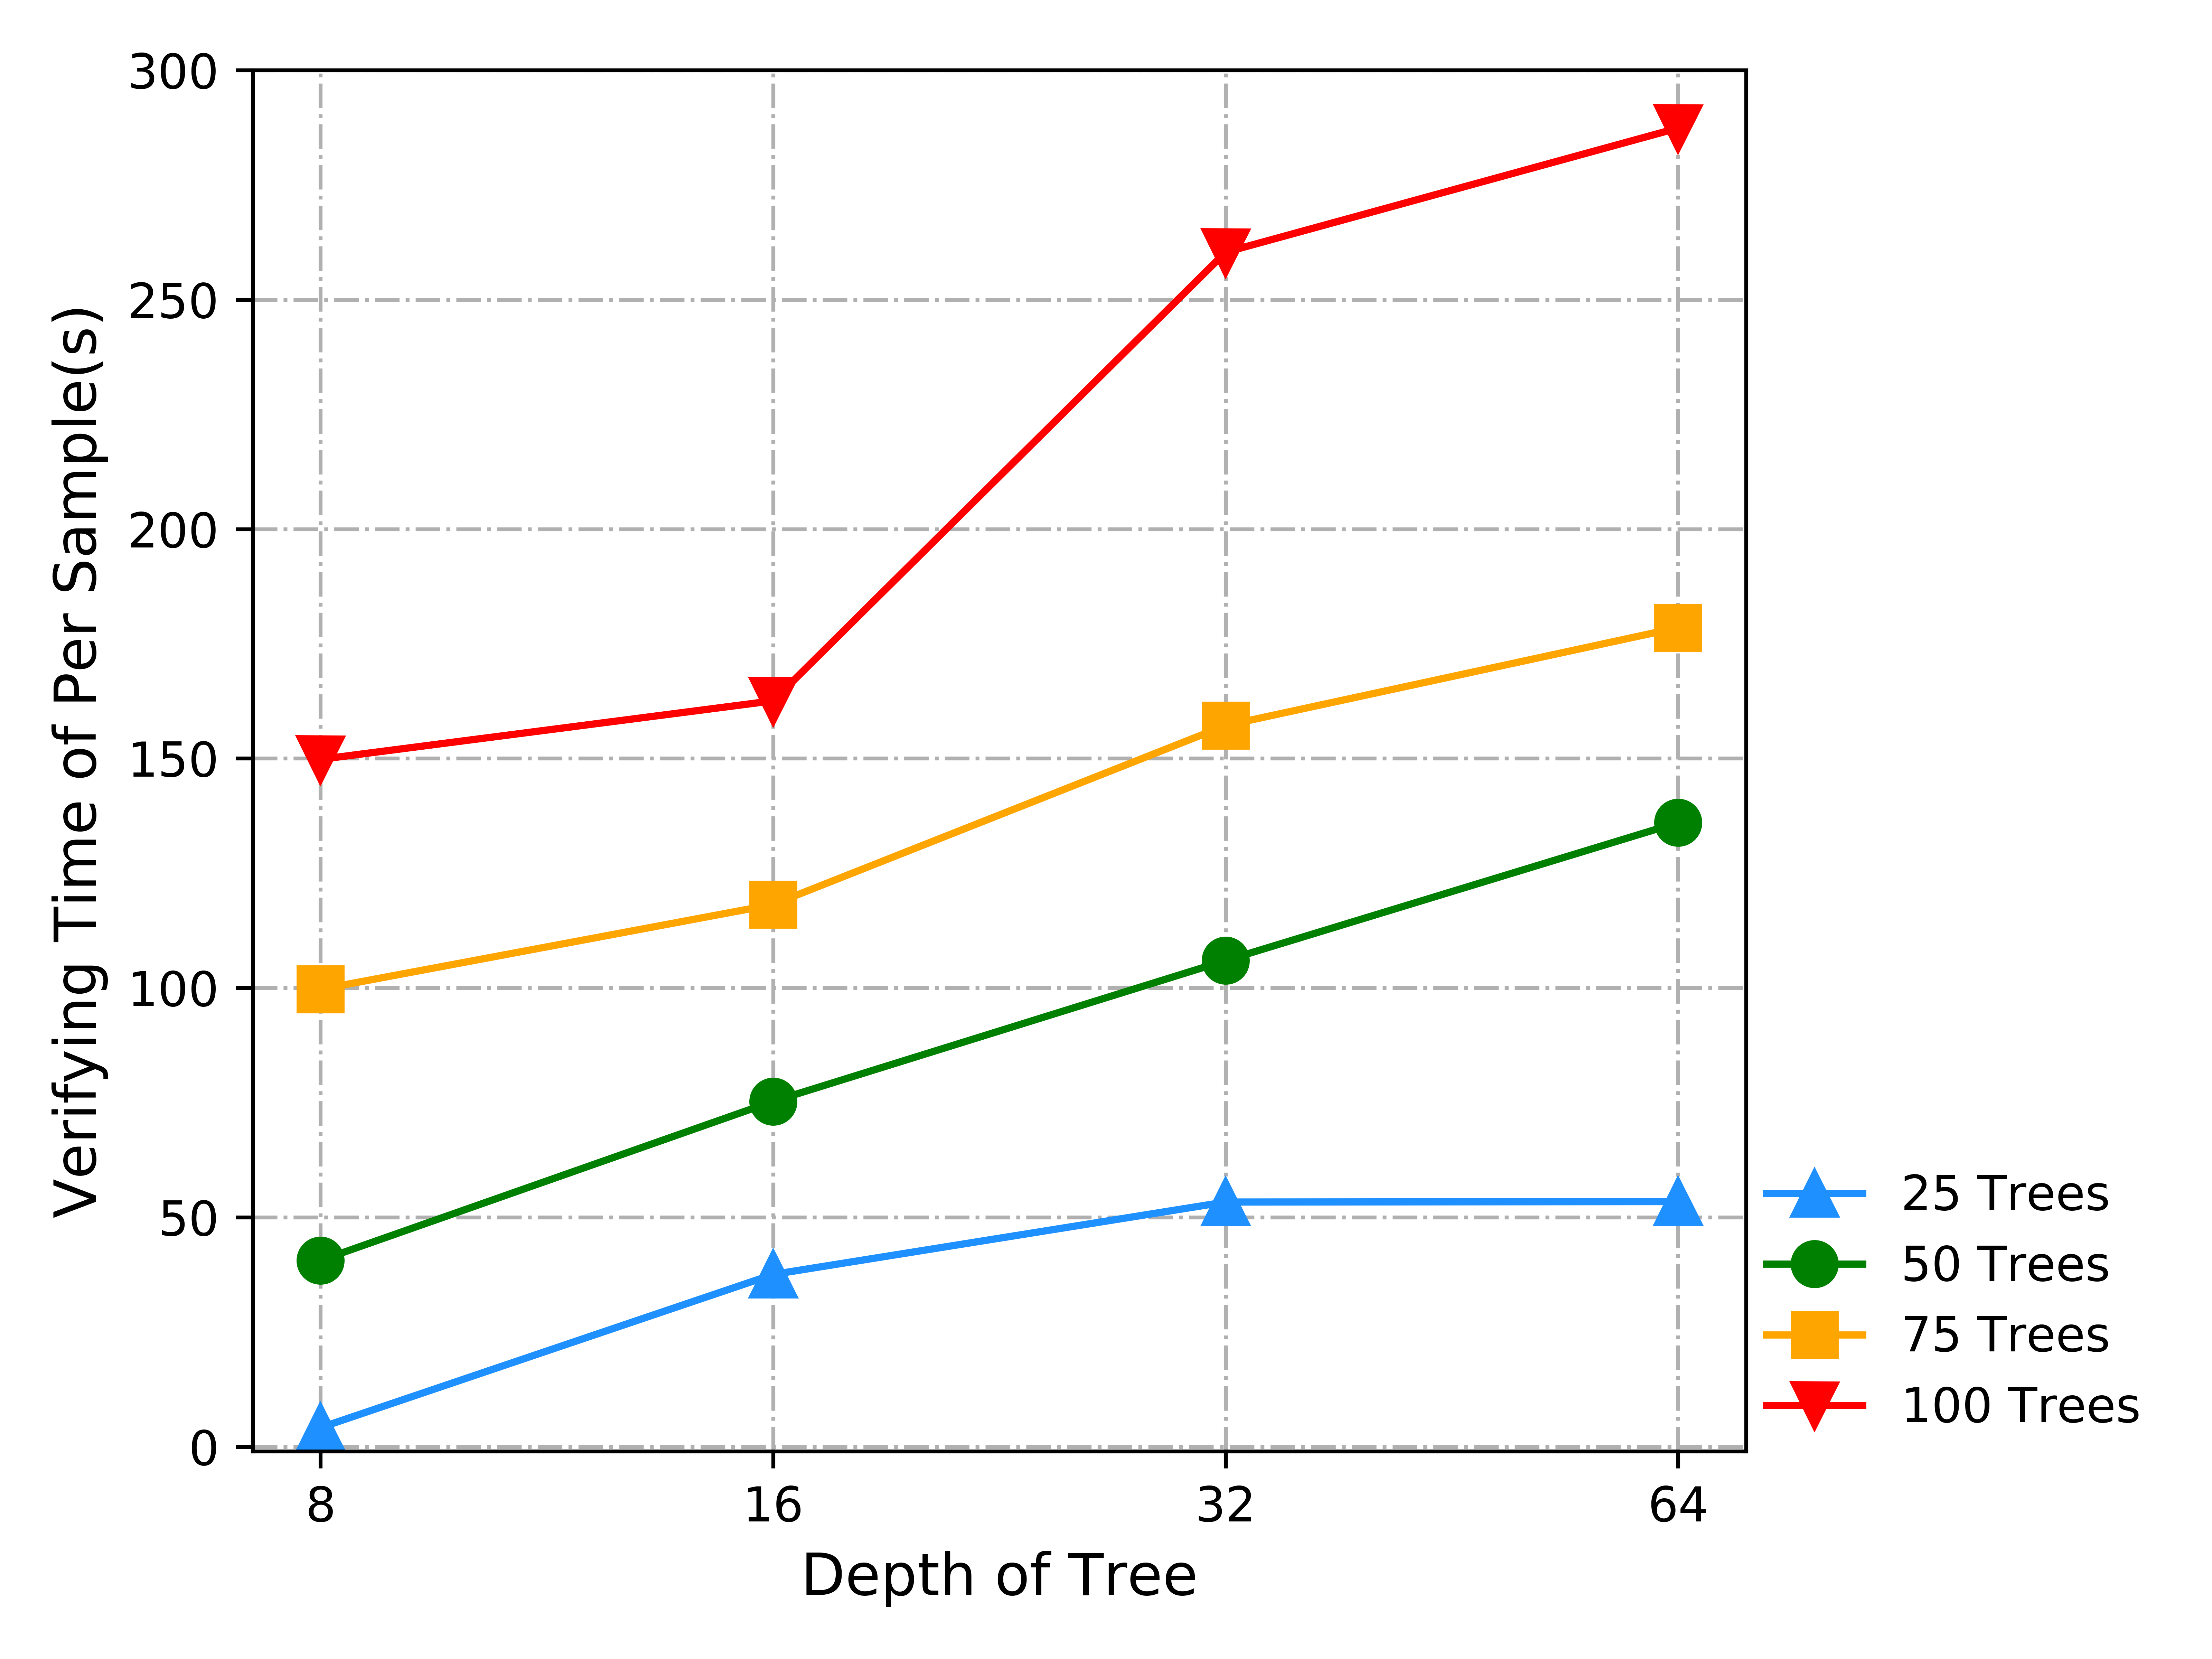
\includegraphics[scale=0.7]{fig2/C5/mnist_time.png}
	\caption{单样本验证时间图}
	\label{fig:mnist_time.png}	
\end{figure}

图\ref{fig:mnist_time.png}为在不同规模树模型下验证单个样本所需要的平均时间统计图。我们在测试样本集中随机选择了 100 个样本来进行验证时间的结果统计,结果值为平均值。我们的验证覆盖了规模很小到大规模的树模型,最小规模为深度为 8, 棵树为 25 的树,单个样本的验证时间4s。 而对于树的棵树为 100,深度为64 的大规模的模型,我们框架的验证时间为287s。随着树模型规模的增加,验证时间也在逐渐增加。总体来说,我们框架可以去验证大规模的树模型的鲁棒性,而且验证时间也是可接受的时间范围。但如表\ref{tab1}所显示的,在进行大规模模型的验证的时候,有些样本可能会出现验证超时的情况,这也是我们在未来工作中,需要解决的问题。

\section{本章小结}
在本章中,我们选取了三个基准数据集对本文提出的鲁棒性验证框架进行了一系列的实验来测试其可行性,并且对树模型鲁棒性的可解释性和树模型训练参数与鲁棒性的关系也进行实验和研究。实验结果表明,我们的验证框架可以有效验证随机森林和 GBDT 这两个树模型的重要组成部分。但也存在不足,就是虽然可以验证大规模的树模型,可是某些样本还是会出现验证超时的情况,这将是我们未来工作中的重点。
